% tex file for discussion
\par \indent Cohen's paper identifies sixteen regions of brain activation 
during the course of the BART study. In particular, we able to detect 
high activity in the dorsal lateral prefrontal cortex and the occipital lobe. 
The prefrontal cortex encompasses the frontal lobe and stores 
the brain's short-term memory as well as the quick decision making processes. 
The occipital lobe can be found in the back part of the brain, and this region
is responsible for processing visual inputs. We were able to consistently detect
the occipital lobe in our analysis. Both active regions are showcased 
for Subject 23 in Figure \ref{fig:clustersub23}.

\begin{figure}[ht]
\centering
	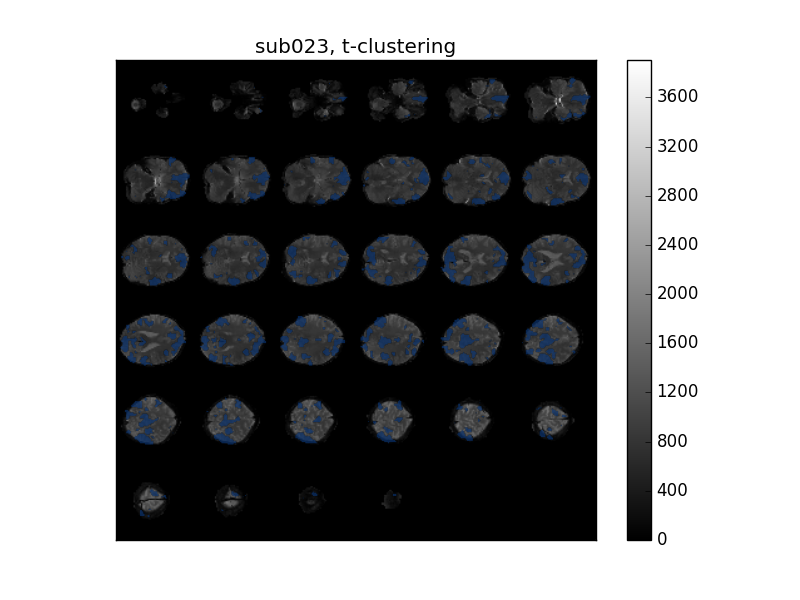
\includegraphics[width=.8\linewidth]{../images/sub023_t_overlay.png} 
	\caption{Quantile-based clustering for Subject 23's t-statistics. 
	(Red areas denote significant regions)}
	\label{fig:clustersub23}
\end{figure}

\par BART studies measure risk-taking behavior, which is a subset of 
self-control. There is activity in both the prefrontal cortex and the 
occipital lobe. This is expected since subjects use visual processing 
centers (the occipital lobe) during the study. While 
visual stimulus is not something that the BART study is interested in 
assessing, it is reasonable that the occipital lobe was nevertheless an site 
of high activity, since there was a strong visual aspect to the study. 
Additionally, subjects utilize 
their short term memory and their decision making during the experiment while
choosing to continue pumping the balloon or cash out. Thus, it makes sense 
that both regions of the brain will be activated during the experiment. 

